
\documentclass[12pt]{article}


\usepackage{placeins}[section]
%% The amssymb package provides various useful mathematical symbols
\usepackage{amssymb}
%% The amsmath package provides various useful equation environments.
\usepackage{amsmath}
%% The amsthm package provides extended theorem environments
%% \usepackage{amsthm}

\usepackage{setspace}
\usepackage{xcolor}
\usepackage[normalem]{ulem}

\usepackage{placeins}
% \usepackage{amsmath}
\usepackage{bm}
% \usepackage{amssymb}
\usepackage[nopatch]{microtype}
\usepackage{booktabs}
\usepackage{mathtools} % Loads amsmath
\usepackage{setspace}
\usepackage{hyperref}
\usepackage{floatrow}

\usepackage{authblk}

\usepackage[authoryear]{natbib}
\setcitestyle{aysep={}} 

% \bibliography{example}
% \bibliographystyle{elsarticle-harv}

\begin{document}



\title{How Swing Model Assumptions Shape Vote-to-Seat Predictions: Evidence from Recent German Elections\thanks{Funded by the Deutsche Forschungsgemeinschaft (DFG, German Research Foundation) – 529544178.}} %% Article title


\author[1]{Lukas F. Stoetzer}
\author[1]{Cornelius Erfort\thanks{Corresponding author: cornelius.erfort@uni-wh.de}}
\author[2]{Hannah Rajski}
\author[2]{Thomas Gschwend}
\author[3]{Simon Munzert}
\author[3]{Elias Koch}

\affil[1]{University Witten/Herdecke}
\affil[2]{University of Mannheim}
\affil[3]{Hertie School, Berlin}

\date{} % Optional: remove date

\maketitle


\begin{abstract}
The 2025 German federal election, marked by political realignments and major electoral reform, presents new challenges for translating vote shares into parliamentary representation. This paper investigates how different assumptions about vote swings affect projections from national trends to district-level outcomes. We focus on comparing uniform swing (identical percentage-point changes across all districts) versus proportional swing (changes relative to baseline support levels), while also testing other variants including piecewise and interaction models that capture how swing behavior varies depending on existing party support levels \citep{wilson2022models}. We use our forecasting model for the 2025 Bundestag election to retrospectively evaluate these approaches across the last eight federal elections (yielding more than 20,000 observations) and complement this empirical analysis with a comprehensive simulation study exploring the parameter space of electoral systems. We compare their accuracy in predicting district vote shares, plurality winners, and—unique to 2025—the likelihood of vacant districts due to electoral reform\footnote{The analysis to assess the implications of swing model choice on the prediction of vacant districts is still in progress.}. Our findings demonstrate that while differences between swing models are generally small, the choice of swing model can meaningfully alter seat projections. The simulation reveals that uniform swing performs better with larger national swings, lower volatility between districts and more parties. The paper contributes to broader debates on electoral forecasting and the mechanics of vote-to-seat translation in proportional systems.

\end{abstract}
\doublespacing

\section{Introduction}

The 2025 German federal election, marked by political realignments and landmark electoral reform, challenges scholars to rethink how votes are translated into parliamentary representation. A critical methodological question emerges: How do different assumptions about vote swings affect projections from national vote shares to district-level outcomes?

Electoral forecasts frequently rely on swing models to translate national polling trends into district-level predictions. These models are widely used in forecasting Congressional elections in the US \citep{bafumi2006forecasting} and parliamentary elections in the UK \citep{fisher2011polls,hanretty2016combining}. Two dominant approaches exist: uniform swing, which assumes identical percentage-point shifts across all districts, and proportional swing, where vote shares change relative to prior support levels—capturing larger shifts in competitive districts and smaller changes in party strongholds. Recognizing the limitations of both approaches, recent research suggests that hybrid swing models, combining elements of uniform and proportional swing, offer more flexible, party-specific adjustments across districts.

Building on our Zweitstimme.org forecasting model for the 2025 Bundestag election \citep{erfort2025zweitstimme,neunhoeffer2020ansatz}, we systematically evaluate uniform swing versus proportional swing as our main comparison, while also testing other variants. Piecewise models, for instance, inspired by recent theoretical work \citep{wilson2022models}, capture the insight that swing behavior may differ depending on existing party support levels—a key advantage that proportional models already attempt to model better than uniform approaches. We apply these approaches retrospectively to the eight most recent federal elections, yielding more than 20,000 observations across 299 districts, assessing their performance in predicting district-level vote shares, plurality winners, and—unique to 2025—the likelihood of vacant districts resulting from electoral reform. We complement this empirical analysis with a comprehensive simulation study that explores the parameter space of electoral systems, systematically varying party system characteristics, electoral volatility, and swing concentration patterns. This dual approach allows us to identify both empirical patterns in German elections and generalizable insights about when different swing assumptions are most appropriate. We show that while differences between swing models are generally small, the choice of swing model can substantially alter seat projections in mixed-member systems, where district outcomes critically shape overall representation.

\newpage
\section{Empirical Analysis}



\subsection{Data and Methodology}

Our empirical analysis uses district-level election results from all eight German federal elections since 1998 (i.e., 1998, 2002, 2005, 2009, 2013, 2017, 2021, and 2025), covering all 299 electoral districts\footnote{Some elections had more districts.}. The dataset contains more than 20,000 observations representing individual candidacies, with ``other candidates" aggregated as a single observation. We employ an out-of-sample forecasting framework where we train our models on seven elections and predict the eighth, rotating through all possible combinations to ensure robust evaluation. This approach mirrors real-world forecasting conditions where models must generalize to unseen electoral contexts.

For each election, we collect district-level vote shares for all parties that received at least 5\% of the national vote or won at least three district seats. The data includes both first votes (for district representatives) and second votes (for party lists). We also incorporate district-level demographic and socioeconomic variables to capture local contextual factors.

Our forecasting models combine national polling trends with district-level historical patterns. We focus on comparing two main approaches: (1) uniform swing models that apply identical percentage-point changes across all districts, and (2) proportional swing models that scale changes relative to baseline support levels. Additionally, we test piecewise interaction variants that capture how swing behavior varies depending on existing party support levels. The piecewise models, building on theoretical insights from \citep{wilson2022models}, allow swing behavior to differ for parties above and below average support levels, capturing the intuition that swing dynamics may vary systematically with baseline party strength. All models are estimated using ordinary least squares regression with district and party fixed effects to account for unobserved heterogeneity.

\subsection{Model Variants}

Our empirical evaluation encompasses ten distinct model specifications, each representing different theoretical assumptions about electoral dynamics. All models include candidate and district-specific covariates to control for systematic factors that influence electoral outcomes beyond national-level swings.

\subsubsection{Candidate and District Covariates}

All models (except pure variants) include the following covariates: \texttt{ncand} (number of candidates in the district), \texttt{propPlatz} (relative measure for the list position), \texttt{alsoList} (indicates whether a candidate also runs on a party list), \texttt{res\_l1\_E} (past first vote share), \texttt{formercand} (whether this candidate already ran in past elections), \texttt{east} (East Germany indicator), \texttt{female} (gender indicator), \texttt{incumbent} (incumbency status), \texttt{akad} (PhD title indicator), \texttt{incumbent\_in\_wkr} (whether the incumbent is running in the district), and \texttt{no\_cand\_l1} (indicator for parties without a candidate in the previous election).

\subsubsection{Swing Model Specifications}

\textbf{Proportional and Uniform Models:} The proportional model uses \texttt{proportional\_swing} (past second vote share plus proportional change), while the uniform model uses \texttt{uniform\_swing} (past second vote share plus uniform change). These models represent the core theoretical distinction between proportional and uniform swing assumptions.

\textbf{Mixed Model:} This specification includes both \texttt{proportional\_swing} and \texttt{uniform\_swing} terms, allowing the regression to find an optimal balance between proportional and uniform components based on the data.

\textbf{Piecewise Models:} Both uniform and proportional piecewise models allow swing effects to differ between districts where a party performed above or below the party's average vote share. This captures the intuition that swing behavior may vary systematically with baseline party strength, as suggested by \citet{wilson2022models}.

\textbf{Pure Models:} These specifications exclude all candidate and district-specific covariates, focusing solely on the swing mechanism. The pure proportional model uses only \texttt{res\_l1\_E} and \texttt{proportional\_swing}, while the pure uniform model uses \texttt{res\_l1\_E} and \texttt{uniform\_swing}.

\textbf{Interaction Models:} Similar to piecewise models but more flexible, these specifications allow for continuous interactions between past vote share and swing coefficients. The proportional interaction model includes \texttt{res\_l1\_Z*proportional\_swing}, while the uniform interaction model includes \texttt{res\_l1\_Z*uniform\_swing}.

\textbf{No Adjustment Model:} This baseline specification contains all candidate and district covariates plus \texttt{res\_l1\_Z} (past second vote share) but excludes any swing component, serving as a control to assess the value added by swing modeling.

\subsection{Empirical Results}

Our empirical analysis reveals that differences between swing models are generally very small, but meaningful patterns emerge across different performance metrics. In terms of district winner prediction accuracy, the differences between the best performing model (mixed swing) and worst performing model (proportional piecewise) amount to less than one percentage point—representing fewer than 3 out of 299 districts. This suggests that for the primary goal of predicting district winners, the choice of swing model has limited practical impact.

However, more substantial differences emerge when examining mean error of vote share predictions. Here, adding interaction terms to both uniform and proportional swing models significantly reduces prediction errors. These interaction terms allow swings to affect districts differently based on prior vote share for a party, capturing the intuition that swing behavior may vary systematically with baseline party strength. This finding aligns with theoretical expectations that more sophisticated models should better capture the heterogeneity of electoral dynamics across districts.

Models also differ substantially in their production of out-of-bounds predictions (vote shares below 0\% or above 100\%). Out-of-bounds predictions occur when swing models predict that a party will receive negative vote shares or more than 100\% of the vote in a district—both physically impossible outcomes that violate the fundamental constraints of electoral systems. These predictions arise when models fail to account for the bounded nature of vote shares or when the relationship between national-level changes and district-level outcomes becomes non-linear.

Pure proportional swing models without covariates for candidate or district-specific characteristics perform worst on this metric, while proportional models with interaction terms perform very well. This suggests that interaction terms not only improve prediction accuracy but also help maintain realistic vote share bounds by capturing the complex, context-dependent relationships between baseline support and swing behavior. While out-of-bounds predictions can technically be handled by truncating them to 0\% or 100\%, this approach is problematic because it distorts the relative relationships between parties and can lead to vote shares that no longer sum to 100\% across all parties in a district. Avoiding out-of-bounds predictions in the first place is therefore crucial for practical electoral forecasting because they can lead to nonsensical seat projections, undermine the credibility of forecasts, and make it impossible to calculate meaningful district-level outcomes that sum to 100\%.

Figure \ref{fig:geographical_mispredicted} shows the geographical distribution of mispredicted electoral districts, i.e. of districts where the actual plurality winner of the candidate vote shares is different than predicted by our model. Mispredicted electoral districts often cluster regionally and by party, indicating that one or more parties perform much better in entire regions than expected. This regional clustering suggests that local factors and party organizational strength play important roles that are not captured by the assumed data generating process of national swing models.

When comparing actual and predicted results for mispredicted electoral districts (Figure \ref{fig:mispredicted_connected_facets}), we observe differences in predictions across models and elections. Notably, in some elections like 2025, predictions of plurality winners in electoral districts assuming uniform swing appears to underperform relative to predictions assuming proportional swing as the triangles are on average further away from the dashed diagonal line than the dots, suggesting that the electoral context may favor different swing assumptions. Additionally, there are more triangles than dots, indicating more mispredicted districts in the uniform model for this election.

The logistic regression results (see Appendix) show small but systematic differences in prediction accuracy. Uniform swing especially performs somewhat better when CDU/CSU is the actual winner, reflecting the historical dominance of this major parties in German politics.

\FloatBarrier

\begin{table}[H]
\centering
\caption{Average, Maximum and Minimum Accuracy of Candidate Vote Share Prediction Models for the Elections 1998, 2002, 2005, 2009, 2013, 2017, 2021, 2025.} 
\label{tab:eval_aggregate}
\begingroup\footnotesize
\begin{tabular}{lrrr}
  \hline \hline 
 \hline
name & avg_accuracy_winner & min_accuracy_winner & max_accuracy_winner \\ 
  \hline
mixed & 0.874 & 0.803 & 0.926 \\ 
  uniform_piecewise & 0.873 & 0.819 & 0.926 \\ 
  uniform & 0.873 & 0.803 & 0.933 \\ 
  proportional_interaction & 0.873 & 0.799 & 0.933 \\ 
  uniform_interaction & 0.869 & 0.806 & 0.930 \\ 
  proportional & 0.869 & 0.793 & 0.926 \\ 
  proportional_piecewise & 0.865 & 0.783 & 0.930 \\ 
  no_adjustment & 0.796 & 0.655 & 0.933 \\ 
   \hline
\end{tabular}
\endgroup
\end{table}


\begin{figure}[h]
    \centering
    \includegraphics[width=\linewidth]{figures/accuracy.pdf}
    \caption{Out-of-sample Performance of Models Across Elections 1998-2025}
    \label{fig:accuracy}
\end{figure}

\begin{figure}[h]
    \centering
    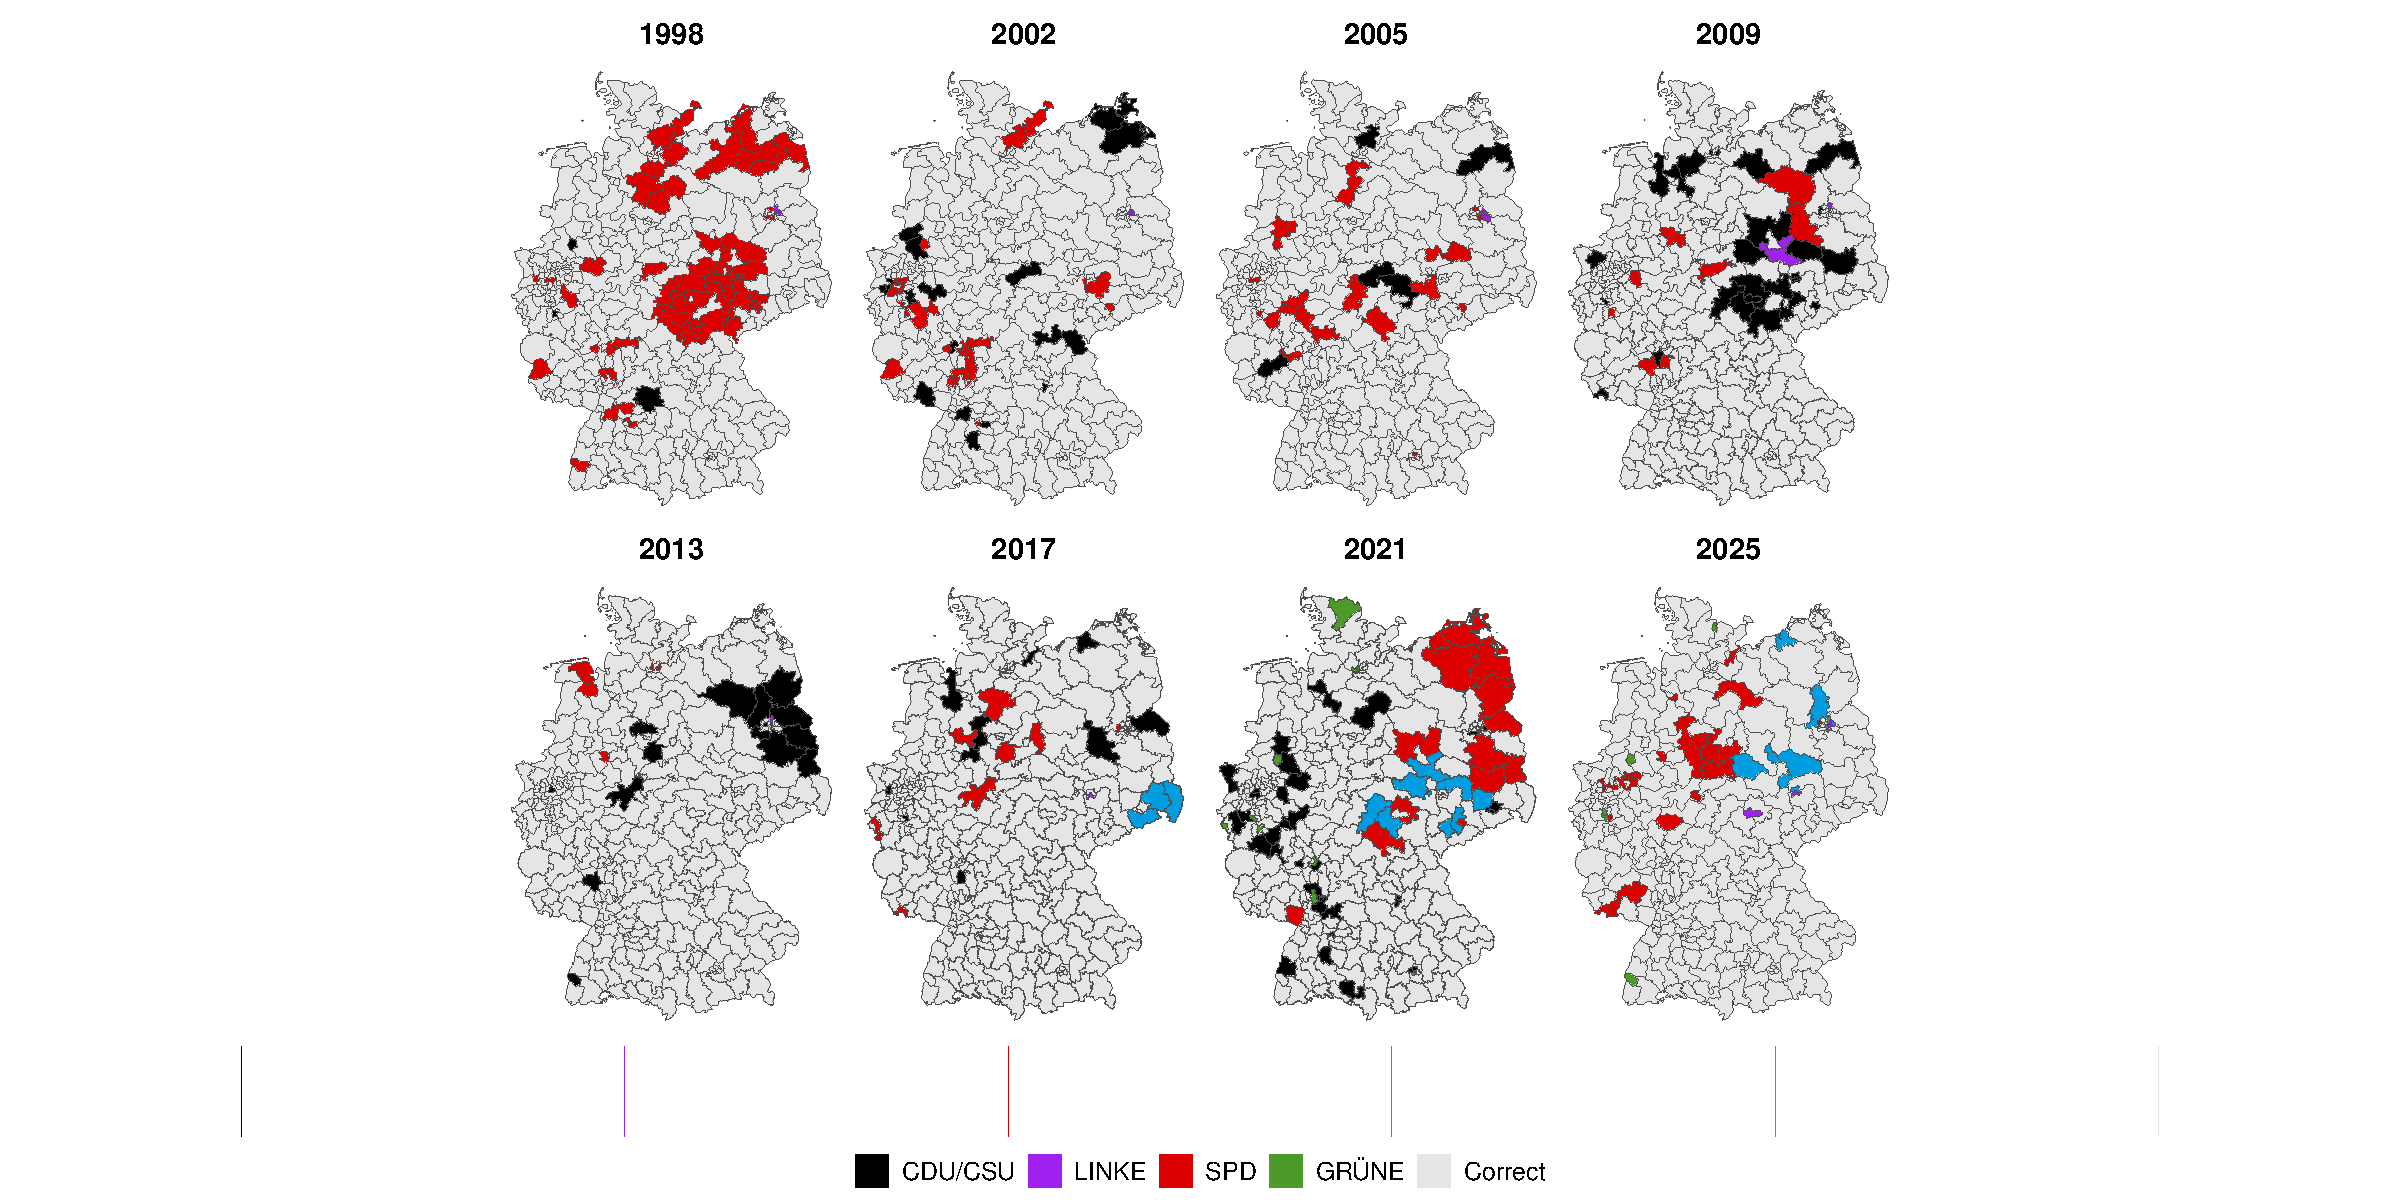
\includegraphics[width=\linewidth,clip,trim = 8cm 0cm 8cm 0 cm]{figures/all_years_incorrect_forecasts.pdf}
    \caption{Geographical distribution of mispredicted districts by election}
    \floatfoot{Note: Predictions based on the model with highest average winner accuracy. Colours show actual winner of mispredicted districts.}
    \label{fig:geographical_mispredicted}
\end{figure}

\begin{figure}[h]
    \centering
    \includegraphics[width=\linewidth,clip,trim = 0cm 0cm 0cm 0 cm]{figures/mispredicted_results_connected_facets.pdf}
    \caption{Actual and Predicted Results for Mispredicted District Winners}
    \floatfoot{Note: Lines connect observations from different models of the same mispredicted electoral district. Shaded areas indicate density of all observations.}
    \label{fig:mispredicted_connected_facets}
\end{figure}





\FloatBarrier

\newpage
\section{Simulation Design and Methodology}

\subsection{Research Objective and Overview}

This simulation study systematically evaluates the performance of uniform versus proportional swing as our main comparison, while also testing a mixed swing variant that combines both approaches. The primary goal is to identify conditions under which each swing assumption performs optimally, providing guidance for real-world electoral forecasting. We employ a comprehensive factorial design that explores the parameter space of electoral systems, generating synthetic data through a realistic data generating process (DGP) that captures the key dynamics of multi-party electoral competition.

\subsection{Data Generating Process}

The simulation employs a realistic data generating process that captures the essential dynamics of electoral systems. Each scenario generates baseline vote shares for 2-7 political parties across 100 districts, with party characteristics varying systematically across the parameter space. Large parties receive baseline support of 25-35\% with district-level variation (standard deviation = 0.08), while small parties receive baseline support of 5-15\% with district-level variation (standard deviation = 0.05). Geographic clustering is modelled through stronghold districts, where specific parties receive elevated support (30-60\% of baseline vote share) in 10-40 designated districts. All vote shares are normalized to sum to 100\% within each district to ensure realistic electoral outcomes.

National-level party vote share changes are drawn from a normal distribution with mean zero and standard deviation varying from 0.01 to 0.09 across scenarios, reflecting different levels of electoral volatility. \textcolor{red}{\textbf{The uniform share parameter (0-1) controls the balance between uniform and proportional swing components in the data generating process. When uniform share equals zero, the simulation generates purely proportional swing behavior, while when it equals one, it generates purely uniform swing behavior. Values in between create hybrid scenarios that combine both approaches. This formulation allows for a continuous spectrum from purely proportional to purely uniform swing behavior, enabling fine-grained analysis of the transition between these assumptions.}}

District-specific noise is added to capture local factors not captured by national trends, with district noise standard deviation varying from 0.002 to 0.03 across scenarios. Large parties receive 1.5 times the district noise of small parties to reflect their greater local variation and organizational capacity. Finally, random noise (standard deviation = 0.01) is added to simulate measurement error and other unpredictable factors that affect real-world electoral outcomes.

\subsection{Model Training and Prediction Framework}

The simulation employs an out-of-sample prediction framework that mirrors real-world electoral forecasting. \textcolor{red}{\textbf{For each scenario, five historical elections are simulated using identical parameters, creating a training dataset with district-party-election observations.}} This training data includes baseline vote shares, actual vote shares, and national swings, providing the foundation for model estimation.

Three models are specified and estimated using ordinary least squares regression on the training data. \textcolor{red}{\textbf{The uniform swing model takes the form: $true\_share \sim uniform\_swing$, the proportional swing model takes the form: $true\_share \sim proportional\_swing$, and the mixed swing model combines both approaches: $true\_share \sim uniform\_swing + proportional\_swing$. In all specifications, the swing variables are pre-calculated using single coefficients that combine baseline support with national-level changes, ensuring that the models learn the true relationship between national-level changes and district-level outcomes without overfitting to interaction terms.}} Our primary focus is on comparing the performance of uniform versus proportional swing models.

A new election is then simulated using the same parameters but different random realizations, serving as the test dataset. The trained models predict district-level vote shares using baseline shares and national swing, and these predictions are compared to true vote shares to assess accuracy. This out-of-sample framework ensures that model performance reflects genuine predictive ability rather than overfitting to the training data.

\subsection{Parameter Space and Experimental Design}

The simulation explores a comprehensive parameter space through a factorial design that systematically varies key electoral system characteristics. The number of parties ranges from 2 to 7, while the number of small parties varies from 0 to 6, capturing different levels of party system fragmentation. Stronghold effects are modelled through 10, 25, or 40 districts with elevated support levels of 30\%, 45\%, or 60\% of baseline vote share.


\begin{figure}[h]
    \centering
    \includegraphics[width=\linewidth]{figures/01_parameter_grid.pdf}
    \caption{Parameter Grid Visualization}
    \label{fig:parameter_grid}
\end{figure}

Electoral volatility is captured through national swing variance ranging from 0.01 to 0.09, while \textcolor{red}{\textbf{the uniform share parameter varies from 0 to 1, allowing for fine-grained analysis of the transition from uniform to proportional swing behavior.}} District-level noise standard deviation ranges from 0.002 to 0.03, reflecting different levels of local unpredictability. This factorial design creates 20,251 unique scenario combinations, \textcolor{red}{\textbf{with five simulations per scenario, resulting in 101,255 total simulations}} that provide robust statistical power for identifying key factors affecting model performance.

\subsection{Performance Evaluation and Analysis}

Performance is evaluated using district winner prediction accuracy, defined as the proportion of districts where the model correctly predicts the winning party, and average errors (MAE and RMSE). These metrics directly correspond to the practical goal of electoral forecasting and provide an intuitive measure of model effectiveness. Our primary analysis compares uniform versus proportional swing models across the parameter space to identify optimal conditions for each approach, with the mixed swing model serving as a reference point for combined approaches.

Statistical analysis employs regression models to identify the factors that explain performance differences between swing assumptions. The dependent variable is the accuracy difference between models, while independent variables include log-transformed parameters and interaction terms. Key variables include the number of parties, number of small parties, swing concentration, and district noise. Separate analyses are conducted for scenarios with few versus many small parties to identify conditional effects.

\subsection{Validation and Empirical Comparison}

To assess the realism of the simulation framework, results are compared to empirical German federal election data covering 299 districts across 8 elections. German parameters are extracted from historical data and used to create a realistic scenario within the simulation framework. This empirical comparison provides a benchmark for assessing whether the simulation captures the essential dynamics of real electoral systems and whether the relative performance of swing models in the simulation aligns with empirical observations.

The simulation framework incorporates several robustness checks to ensure reliable results. Parameter ranges are chosen to span realistic electoral contexts, multiple simulations per scenario assess robustness to random variation, and the comprehensive parameter space exploration identifies boundary conditions where model performance may change dramatically. This systematic approach provides confidence that the findings generalize across diverse electoral contexts and are not artifacts of specific parameter choices.

\subsection{Key Innovations and Contributions}

Our simulation framework introduces several methodological innovations that advance the study of electoral forecasting. The realistic DGP incorporates both uniform and proportional swing components, models geographic clustering through stronghold effects, and captures party size differences in baseline support and variation. The out-of-sample prediction framework mirrors real-world forecasting conditions, where models must generalize to unseen data, avoiding the overfitting that can occur when models are evaluated on the same data used for training.

The systematic parameter variation through factorial design enables identification of key factors affecting model performance, while the continuous swing concentration parameter allows for fine-grained analysis of the transition between swing assumptions. The comprehensive coverage of electoral system characteristics ensures that findings are relevant across diverse contexts, from stable two-party systems to volatile multi-party environments. This simulation framework provides a rigorous foundation for understanding when different swing assumptions are most appropriate, offering practical guidance for electoral forecasting across diverse contexts.

\subsection{Simulation Results}

Our simulation study, exploring 20,251 unique scenario combinations, reveals that overall differences between swing models remain small, which could be attributed to the fact that we always train the models on empirical data. If 100\% proportional swing would, for example, be too extreme, the models automatically down-correct.

Our analysis reveals that while the mixed swing model generally performs best overall, the relative performance of uniform versus proportional swing varies systematically with party system characteristics. Proportional swing performs better in systems with more small parties (i.e., parties receiving baseline support of 5-15\%), while uniform swing shows advantages in systems with higher numbers of parties and greater electoral volatility. This finding aligns with the theoretical expectation that proportional swing should better capture the dynamics of multi-party competition, while uniform swing may be more robust in volatile, multi-party environments.

The key interaction effects (Figure \ref{fig:key_interaction}) highlight the important interaction between the number of parties and the number of small parties. Increasing the number of parties tends to give uniform swing an advantage, but with increasing numbers of small parties, proportional swing performs better. This finding suggests that party system fragmentation affects the optimal choice of swing assumption.

The regression analysis of all scenarios (Figure \ref{fig:regression_coefficients}) reveals several systematic patterns in model performance. First, the uniform share parameter in the DGP significantly increases the advantage of uniform swing models, which is expected since higher uniform share means the data generating process more closely resembles uniform swing behavior. This effect is particularly evident in the first differences plot (Figure \ref{fig:first_differences}), which standardizes effects by showing the change in model performance when moving from the minimum to maximum value of each parameter, making effects comparable across different parameter scales and ranges.

Second, higher national vote variance (capturing electoral volatility) actually makes proportional swing models perform better. This counterintuitive finding can be explained by the DGP structure: when national-level changes are large, the proportional swing model's ability to scale changes relative to baseline support becomes more valuable, as it can better capture the heterogeneous impact of large national swings across districts with different baseline party strengths.

Third, higher district vote volatility (district noise) makes uniform swing models perform better. This pattern emerges because when local factors dominate (high district noise), the uniform swing model's assumption of identical changes across districts becomes more robust. The proportional model, which relies on baseline support levels to predict swing behavior, becomes less reliable when district-specific factors introduce substantial variation that masks the systematic relationship between baseline support and swing magnitude.







\begin{figure}[h]
    \centering
    \includegraphics[width=\linewidth]{figures/04_key_interaction.pdf}
    \caption{Key Interaction Effects}
    \label{fig:key_interaction}
\end{figure}

\begin{figure}[h]
    \centering
    \includegraphics[width=\linewidth]{figures/05_regression_coefficients.pdf}
    \caption{Regression Coefficients Analysis}
    \label{fig:regression_coefficients}
\end{figure}

\begin{figure}[h]
    \centering
    \includegraphics[width=\linewidth]{figures/06_first_differences.pdf}
    \caption{First Differences Analysis: Standardized Effects on Model Performance}
    \label{fig:first_differences}
\end{figure}

% 
% Table created by stargazer v.5.2.3 by Marek Hlavac, Social Policy Institute. E-mail: marek.hlavac at gmail.com
% Date and time: Tue, Aug 12, 2025 - 17:05:52
\begin{table}[!htbp] \centering 
  \caption{Model Performance by Party Configuration} 
  \label{} 
\begin{tabular}{@{\extracolsep{5pt}} cccccccccccccccc} 
\\[-1.8ex]\hline 
\hline \\[-1.8ex] 
 & n\_parties & n\_small\_parties & n\_scenarios & uniform\_better\_acc & proportional\_better\_acc & avg\_accuracy\_diff & uniform\_better\_mae & proportional\_better\_mae & avg\_mae\_diff & uniform\_better\_rmse & proportional\_better\_rmse & avg\_rmse\_diff & better\_model\_acc & better\_model\_mae & better\_model\_rmse \\ 
\hline \\[-1.8ex] 
1 & 2 & 0 & 30 & NA & NA & NaN & NA & NA & NaN & NA & NA & NaN & Equal & Equal & Equal \\ 
2 & 3 & 0 & 30 & 15 & 14 & -0.000148110736999626 & 15 & 15 & 1.37329873045299e-06 & 17 & 13 & -7.87378827707361e-06 & Uniform & Equal & Uniform \\ 
3 & 3 & 2 & 30 & 0 & 0 & 0 & 17 & 13 & -1.66894850381856e-05 & 17 & 13 & -3.84202743255286e-05 & Equal & Uniform & Uniform \\ 
4 & 4 & 0 & 30 & 23 & 5 & 0.000548262695685394 & 26 & 4 & -1.19054627993549e-05 & 28 & 2 & -1.81984172774687e-05 & Uniform & Uniform & Uniform \\ 
5 & 4 & 2 & 30 & 3 & 27 & -0.00204814814814814 & 15 & 15 & 1.06525606150203e-05 & 8 & 22 & 5.34921251645448e-05 & Proportional & Equal & Proportional \\ 
6 & 5 & 0 & 30 & 30 & 0 & 0.00242871283322762 & 30 & 0 & -3.3979078708065e-05 & 29 & 1 & -5.81324452678357e-05 & Uniform & Uniform & Uniform \\ 
7 & 5 & 2 & 30 & 9 & 20 & -0.000588888888888898 & 17 & 13 & -8.78004545669388e-07 & 9 & 21 & 1.86684395590164e-05 & Proportional & Uniform & Proportional \\ 
8 & 5 & 4 & 30 & 1 & 29 & -0.00261481481481482 & 8 & 22 & 4.13377604293099e-05 & 5 & 25 & 8.43642132545452e-05 & Proportional & Proportional & Proportional \\ 
9 & 6 & 0 & 30 & 26 & 2 & 0.00205559296670409 & 26 & 4 & -5.57987069485659e-05 & 30 & 0 & -8.72975146536367e-05 & Uniform & Uniform & Uniform \\ 
10 & 6 & 2 & 30 & 23 & 5 & 0.00137407407407407 & 22 & 8 & -2.04787631722332e-05 & 28 & 2 & -3.55963081299299e-05 & Uniform & Uniform & Uniform \\ 
11 & 6 & 4 & 30 & 14 & 16 & -0.00028888888888889 & 10 & 20 & 2.00961231460091e-05 & 11 & 19 & 2.19507227141147e-05 & Proportional & Proportional & Proportional \\ 
12 & 7 & 0 & 30 & 30 & 0 & 0.00290370370370372 & 26 & 4 & -6.40667221506769e-05 & 30 & 0 & -0.000122818369685815 & Uniform & Uniform & Uniform \\ 
13 & 7 & 2 & 30 & 28 & 2 & 0.00149259259259259 & 30 & 0 & -4.46791579808118e-05 & 30 & 0 & -7.92650319345875e-05 & Uniform & Uniform & Uniform \\ 
14 & 7 & 4 & 30 & 23 & 7 & 0.00103703703703704 & 21 & 9 & -1.55709106688259e-05 & 25 & 5 & -3.0853560578064e-05 & Uniform & Uniform & Uniform \\ 
15 & 7 & 5 & 1 & 1 & 0 & 0.005 & 1 & 0 & -2.98669884639738e-05 & 1 & 0 & -0.000220022701123236 & Uniform & Uniform & Uniform \\ 
16 & 7 & 6 & 30 & 12 & 18 & -0.000211111111111118 & 14 & 16 & 7.06219283094269e-06 & 11 & 19 & 1.0816176316449e-05 & Proportional & Proportional & Proportional \\ 
\hline \\[-1.8ex] 
\end{tabular} 
\end{table} 


% 
% Table created by stargazer v.5.2.3 by Marek Hlavac, Social Policy Institute. E-mail: marek.hlavac at gmail.com
% Date and time: Thu, Jan 29, 2026 - 13:12:39
\begin{table}[!htbp] \centering 
  \caption{Regression Results: Explaining Model Performance Differences} 
  \label{} 
\begin{tabular}{@{\extracolsep{5pt}}lccc} 
\\[-1.8ex]\hline 
\hline \\[-1.8ex] 
\\[-1.8ex] & Uniform - Proportional & Uniform - Proportional & Uniform - Proportional \\ 
 & Accuracy Diff & MAE Diff & RMSE Diff \\ 
\\[-1.8ex] & (1) & (2) & (3)\\ 
\hline \\[-1.8ex] 
 log\_n\_parties & 0.0042$^{***}$ & $-$0.0033$^{***}$ & $-$0.0049$^{***}$ \\ 
  & (0.0003) & (0.0000) & (0.0000) \\ 
  & & & \\ 
 log\_n\_small\_parties & $-$0.0000 & 0.0004$^{***}$ & 0.0008$^{***}$ \\ 
  & (0.0002) & (0.0000) & (0.0000) \\ 
  & & & \\ 
 stronghold\_ratio & 0.0002 & $-$0.0000 & $-$0.0000 \\ 
  & (0.0007) & (0.0001) & (0.0001) \\ 
  & & & \\ 
 log\_national\_level\_vote\_variance & $-$0.0235$^{***}$ & 0.0078$^{***}$ & 0.0113$^{***}$ \\ 
  & (0.0006) & (0.0001) & (0.0001) \\ 
  & & & \\ 
 uniform\_share & 0.0237$^{***}$ & $-$0.0090$^{***}$ & $-$0.0096$^{***}$ \\ 
  & (0.0003) & (0.0000) & (0.0000) \\ 
  & & & \\ 
 log\_between\_district\_vote\_volatility & 0.0147$^{***}$ & $-$0.0048$^{***}$ & $-$0.0055$^{***}$ \\ 
  & (0.0004) & (0.0000) & (0.0001) \\ 
  & & & \\ 
 small\_stronghold\_ratio & 0.0001 & $-$0.0000 & $-$0.0000 \\ 
  & (0.0005) & (0.0001) & (0.0001) \\ 
  & & & \\ 
 Constant & $-$0.0438$^{***}$ & 0.0182$^{***}$ & 0.0275$^{***}$ \\ 
  & (0.0015) & (0.0002) & (0.0002) \\ 
  & & & \\ 
Observations & 152,460 & 152,460 & 152,460 \\ 
R$^{2}$ & 0.0651 & 0.4331 & 0.4539 \\ 
Adjusted R$^{2}$ & 0.0650 & 0.4331 & 0.4539 \\ 
Residual Std. Error (df = 152452) & 0.0339 & 0.0039 & 0.0043 \\ 
F Statistic (df = 7; 152452) & 1,515.5140$^{***}$ & 16,641.0300$^{***}$ & 18,103.3800$^{***}$ \\ 
\hline \\[-1.8ex] 
\textit{Notes:} & \multicolumn{3}{l}{$^{***}$Significant at the 1 percent level.} \\ 
 & \multicolumn{3}{l}{$^{**}$Significant at the 5 percent level.} \\ 
 & \multicolumn{3}{l}{$^{*}$Significant at the 10 percent level.} \\ 
\end{tabular} 
\end{table} 


\FloatBarrier
\newpage
\section{Discussion}

This study provides both empirical and theoretical insights into the performance of different swing model assumptions in electoral forecasting. Our findings contribute to the broader literature on vote-to-seat translation and offer practical guidance for electoral forecasting.

\subsection{Key Findings and Implications}

Our empirical analysis of German federal elections, based on more than 20,000 observations across eight elections and 299 districts, reveals that differences between uniform and proportional swing models are generally small but meaningful. The regional clustering of misclassifications suggests that local factors and party organizational strength play important roles that national swing models cannot fully capture. This finding aligns with previous research emphasizing the importance of local context in electoral outcomes \citep{}. The observation that uniform swing performs better for major parties (CDU/SPD) while proportional swing shows advantages in certain electoral contexts (like 2025) suggests that the optimal swing assumption may vary depending on the specific electoral environment and party system configuration.

The simulation results provide broader theoretical insights into when different swing assumptions are most appropriate. The finding that uniform swing performs better with higher numbers of parties and higher electoral volatility challenges the conventional wisdom that proportional swing is always superior in multi-party systems. This suggests that the relationship between party system fragmentation and optimal swing assumptions is more complex than previously understood. The interaction between the number of parties and the number of small parties is particularly important, indicating that it's not just the total number of parties that matters, but their relative size distribution. The mixed swing model's superior overall performance suggests that combining uniform and proportional approaches may be optimal in many electoral contexts, though the relative weights may vary systematically with party system characteristics.

\subsection{Theoretical Contributions}

Our study makes several theoretical contributions to the literature on electoral forecasting and vote-to-seat translation. First, we demonstrate that the choice between uniform and proportional swing is not simply a matter of electoral system type, but depends on specific characteristics of the party system and electoral context. This nuanced understanding moves beyond the binary distinction often made in the literature between majoritarian and proportional systems.

Second, our simulation framework introduces a more sophisticated approach to understanding swing model performance. By systematically varying electoral system parameters, we can identify the specific conditions under which each swing assumption performs optimally. This approach provides a foundation for future research on electoral forecasting across diverse contexts.

Third, our findings on the importance of stronghold effects and district-level noise contribute to the growing literature on geographic clustering in electoral behavior. The systematic parameter variation in our simulation framework allows us to identify how these factors interact with swing model performance across diverse electoral contexts.

\subsection{Practical Implications for Electoral Forecasting}

The practical implications of our findings are significant for electoral forecasting in mixed-member proportional systems. Our results suggest that forecasters should consider the specific characteristics of the party system when choosing swing assumptions. In systems with many small parties, proportional swing may be more appropriate, while in systems with high electoral volatility or strong geographic clustering, uniform swing may perform better.

The finding that differences between swing models are generally small suggests that the choice of swing assumption may be less critical than other aspects of the forecasting model, such as the quality of polling data or the inclusion of local contextual factors. However, the systematic patterns we identify suggest that careful consideration of swing assumptions can still improve forecast accuracy, particularly in close elections where small differences matter.

For the 2025 German federal election specifically, our findings suggest that the electoral reform and changing party system dynamics may favor proportional swing assumptions. The underperformance of uniform swing in 2025 relative to proportional swing could reflect the increasing fragmentation of the German party system and the emergence of new political forces.

\subsection{Limitations and Future Research}

Several limitations of our study should be acknowledged. First, our empirical analysis focuses on German elections, and while our simulation provides broader insights, the generalizability of our findings to other contexts requires further testing. Second, our simulation framework, while comprehensive, necessarily simplifies some aspects of real electoral systems. Future research could incorporate more complex party dynamics, such as coalition formation and strategic voting.

Third, our analysis focuses on district-level outcomes, but the ultimate goal of electoral forecasting is often to predict overall parliamentary composition. Future research could examine how different swing assumptions affect seat projections at the national level, particularly in systems with complex seat allocation rules.

Finally, while our simulation includes a mixed swing model that combines uniform and proportional approaches, we focus our main analysis on the comparison between uniform and proportional swing models. Future research could explore more sophisticated hybrid models that adapt to specific electoral conditions and systematically vary the optimal combination of uniform and proportional elements.

\subsection{Conclusion}

This study demonstrates that the choice of swing model assumption in electoral forecasting is more nuanced than previously understood. While differences between uniform and proportional swing are generally small, systematic patterns emerge that can guide forecasters in choosing appropriate assumptions for specific electoral contexts. Our findings suggest that the optimal swing assumption depends on party system characteristics, electoral volatility, and geographic clustering patterns.

The combination of empirical analysis and systematic simulation provides both country-specific insights and generalizable theoretical contributions. For German elections, our results suggest that the changing party system may favor proportional swing assumptions, while the simulation reveals broader patterns that could apply to other mixed-member proportional systems. The systematic exploration of the parameter space provides insights into when different swing assumptions are most appropriate.

Future research should build on these findings to develop more sophisticated forecasting models that can adapt to different electoral contexts and incorporate local factors more effectively. The systematic approach developed in this study provides a foundation for such research and contributes to the broader goal of improving electoral forecasting accuracy across diverse democratic systems.





\newpage
\bibliographystyle{apalike}
\bibliography{references}


\clearpage

\newpage
\appendix

\section{Empirical Analysis: Detailed Results}

\subsection{Regression Coefficient Plots}

The following figures provide detailed coefficient plots from our regression analyses. While the main text summarizes the key findings, these visualizations show the specific effects of different variables on model performance.

\begin{figure}[h]
    \centering
    \includegraphics[width=\linewidth,clip,trim = 0cm 0cm 0cm 0 cm]{figures/coefplot_correct_comparison_custom.pdf}
     \caption{Results from logistic regression: Probability for correct prediction}
     \floatfoot{Note: Brandenburg as state, AfD as party, and 1998 as election year are the excluded reference categories.}
    \label{fig:logistic_regression_appendix}
\end{figure}

\begin{figure}[h]
    \centering
    \includegraphics[width=\linewidth,clip,trim = 0cm 0cm 0cm 0 cm]{figures/coefplot_error_comparison_custom.pdf}
    \caption{Results from linear regression: Size of absolute error (winners only)}
    \floatfoot{Note: Brandenburg as state, and 1998 as election year are the excluded reference categories.}
    \label{fig:linear_regression_winners_appendix}
\end{figure}

\begin{figure}[h]
    \centering
    \includegraphics[width=\linewidth,clip,trim = 0cm 0cm 0cm 0 cm]{figures/coefplot_error_mispredicted_comparison_custom.pdf}
    \caption{Results from linear regression: Size of absolute error (mispredicted winners only)}
        \floatfoot{Note: Brandenburg as state, and 1998 as election year are the excluded reference categories.}
    \label{fig:linear_regression_mispredicted_appendix}
\end{figure}

\section{Declaration of Generative AI Use}

\textbf{Declaration of generative AI and AI-assisted technologies in the writing process}. During the preparation of this work the authors used ChatGPT 4o in order to copy-edit written paragraphs of text. After using this tool/service, the authors reviewed and edited the content as needed and take full responsibility for the content of the publication.


\end{document}